\documentclass[
	12pt,
	oneside,
	a4paper,
	english,
	brazil
]{abntex2}

\usepackage{lmodern}
\usepackage[T1]{fontenc}
\usepackage[utf8]{inputenc}
\usepackage{indentfirst}
\usepackage{color}
\usepackage{graphicx}
\usepackage{microtype}
\usepackage{amsfonts}
\usepackage{csquotes}

\usepackage{tikz}
\usetikzlibrary{positioning}

\usepackage{caption}

\usepackage[brazilian,hyperpageref]{backref}
\usepackage[alf]{abntex2cite}

\usepackage{macros}

\titulo{Previsão de séries temporais por meio de aprendizado de máquina}
\autor{Guilherme Chichanoski}
\local{Maringá}
\data{2018}
\orientador{Valéria Delisandra Feltrim}
\instituicao{Universidade Estadual de Maringá\\
Centro de Tecnologia --- Departamento de Informática\\
Bacharelado em Ciência da Computação}
\tipotrabalho{Trabalho de Conclusão de Curso}

\preambulo{Trabalho de Conclusão de Curso de Graduação apresentado ao 
Departamento de Informática da Universidade Estadual de Maringá, como requisito 
parcial para obtenção do grau de Bacharel em Ciência da Computação.}

\makeatletter
\hypersetup{
		pdftitle={\@title},
		pdfauthor={\@author},
		pdfsubject={\imprimirpreambulo},
		pdfcreator={LaTeX with abnTeX2},
		pdfkeywords={abnt}{latex}{abntex}{abntex2}{projeto de pesquisa},
		colorlinks=true,	% false: boxed links; true: colored links
		linkcolor=blue,		% color of internal links
		citecolor=blue,		% color of links to bibliography
		filecolor=magenta,	% color of file links
		urlcolor=blue,
		bookmarksdepth=4
}
\makeatother

\setlength{\parindent}{1.3cm}
\setlength{\parskip}{0.2cm}

\begin{document}

\frenchspacing

\imprimircapa{}

\imprimirfolhaderosto{}

\textual{}

\pdfbookmark[0]{\contentsname}{toc}
\tableofcontents*
\cleardoublepage{}

\chapter{Introdução}

Segundo \citeonline{wiley} prever é a tarefa de predizer valores futuros ou 
eventos. Essa tarefa pode não ser trivial considerando que autores e 
organizações famosas já incorreram e ainda incorrem em previsões que se 
demonstram erradas, como exemplo podemos citar The New York Times que previu em 
1966 que em 2000 existiriam somente 220.000 computadores no Estados Unidos. A 
tarefa de prever é de grande importância para diversos setores incluindo 
governos e industrias, e sendo a atividade de previsão crucial para o apoio a 
tomada de decisão é evidente a necessidade de se realizar boas previsões.

Ainda segundo \citeonline{wiley} as previsões são classificas como sendo de 
curto, médio e longo prazo.  Sendo as de curto prazo previsões de um futuro 
próximo, ou seja, somente poucos passos a frente, podendo esses passos serem 
contados em dias, semanas ou meses.  Já previsões de médio prazo podem se 
estender por períodos de até um ano no futuro com os passos podendo ser dados em 
meses, enquanto que prazos mais longos serão chamados de previsões de longo 
prazo. Ainda conforme o autor, previsões de médio e longo prazo são mais 
difíceis e suscetíveis a fatores externos.

Para exemplificar a tarefa de previsão de curto prazo podemos citar a atividade 
de previsão da produção de energia eólica, como disposto em 
\citeonline{giebel2011state} a disponibilidade da energia produzida é dada 
segundo a capacidade do vento na região instalada, o vento no entanto é um 
elemento volátil e sendo assim se faz necessário se preparar para possíveis 
momentos quais se farão necessários o uso de outras fontes de energia, essa 
tarefa no entanto pode demandar conhecimento prévio pois o ligamento de uma 
usina como aquelas movidas a diesel podem levar até duas horas. Percebe-se então 
que a tarefa de prever duas horas a frente pode ser crucial para garantir o 
abastecimento de energia a uma região.

% FIXME: Tá esquisito
E em se tratando de previsões, uma fonte de informação comumente utilizado são 
as séries temporais, segundo \citeonline{wiley} essas séries são compostas de 
observações sequenciais ao longo do tempo. Por exemplo podemos observar o 
exemplo de série na \autoref{serie0}. Sendo essas observações separadas 
unicamente pelo tempo pode-se obter os dados em diferentes intervalos, como 
observações diárias, semanais ou ainda anuais.

\begin{figure}[ht]
    \centering
    \caption{Série gerada para exemplo}\label{serie0}
    \includegraphics[width=.6\linewidth]{images/serie_exemplo.png}
    \source{Elaborado pelo autor}
\end{figure}

Tais séries possuem comportamento tal que permite a elaboração de um modelo que 
o representa de forma a permitir previsões, sendo os modelos estatísticos 
considerados os modelos mais comuns para esta finalidade. Como exemplo de 
aplicação podemos citar \citeonline{artigoEx1}, que obteve bons resultados em 
previsões de curto ao empregar modelos probabilísticos. Também vale a citar os 
resultados obtidos por \citeonline{artigoEx2}, no qual também se empregou tais 
modelos e se obteve um modelo suficiente para realizações de previsões.

Em contrapartida podemos citar técnicas de aprendizado de máquinas que estão se 
tornando cada vez mais notórias pelos bons resultados que obtêm, como exemplo 
podemos citar o artigo de \citeonline{artigoEx3} no qual a aplicação de modelos 
utilizando aprendizado de máquina possibilitou a previsão com bons resultados.  
Pelo fato dos modelos estatísticos serem considerados quase um padrão para tais 
modelagens é comum que trabalhos como de \citeonline{artigoEx4} compare os 
resultados obtidos de modelos aprendizado com modelos de abordagem estatísticas.  
No caso dos modelos de aprendizado podemos citar como as redes neurais 
artificiais como sendo capaz de obter bons resultados conforme analisado por 
\citeonline{zhang}, o autor ainda apresenta outros exemplos nos quais a 
utilização de redes neurais obtiveram resultados superiores, considerando ainda 
que o estudo já está datado podemos encontrar em publicações recentes resultados 
ainda melhores considerando os recentes avanços realizados na área de redes 
neurais artificias.

A relevância das previsões são percebidas em aplicações nas quais esta é 
aplicada diretamente no processo de tomada de decisão, podendo auxiliar desde a 
organização de um negócio ao entendimento do comportamento de uma população.

\section{Previsão}
Segundo \citeonline{wiley} podemos separar o processo de previsão em diversas 
atividades, colocadas e detalhadas a seguir:

\begin{itemize}
	\item Definição do problema\\
		Envolve definir e entender a tarefa de previsão a ser realizada,
		considerando o prazo a ser previsto e definindo os dados necessários e
		quanto será o intervalo de uma previsão e outra.
	\item Coleta dos dados\\
		Conforme definido na etapa anterior ocorrerá nessa atividade a coleta
		dos dados.
	\item Análise dos dados\\
		Atividade de alta importância para a seleção do modelo mais adequado,
		nessa etapa é utilizada de observações gráficas e extração de dados para
		identificar padrões que ajudem. Ainda ocorrerá a identificação de 
		observações problemáticas e marcadas.
	\item Seleção e verificação do modelo\\
		Consiste da seleção e verificação de como o modelo escolhido se comporta 
		com os dados fornecidos. Para verificar o comportamento será utilizado 
		métricas que permitam comparar o resultado obtidos com outros modelos.
	\item Avaliação do modelo\\
		Etapa para avaliar como o modelo se comportará com novos dados obtidos, 
		normalmente é realizado a partir de dados separados obtidos das mesmas 
		informações utilizada em etapas anteriores, porem uma parte separada 
		somente para este fim.
	\item Publicação do modelo\\
		Com o modelo devidamente selecionado e avaliado o processo é instalado 
		em ambiente de produção, tendo que observar as alterações necessárias 
		para que novos dados sejam inseridos corretamente.
	\item Monitoramento da performance do modelo\\
		Uma ultima atividade que ocorrerá de forma recorrente, deve-se 
		continuamente avaliar como o modelo aplicado se comporta em relação ao 
		ambiente, já que o ambiente é algo volátil.
\end{itemize}

Vale-se notar que após a tarefa de avaliação se essa resultar em um valor 
insatisfatório deve-se retornar a fase anterior e refeita a avaliação até que um 
modelo que obedeça as especificações seja encontrado.

\chapter{Fundamentação teórica}
A descrição dos fundamentos aplicados neste trabalho se organizará partindo do 
entendimento de séries temporais, explicando o conceito e como são descritas e 
seguirá detalhando modelos probabilísticos, em especial o modelo ARIMA\@. Após 
descrita a parte estatística é descrito os modelos de aprendizado de máquina com 
enfase nos modelos de redes neurais, sendo mais especifico sobre redes 
recorrentes chamadas de LSTM (\textit{Long Short Term Memory}).

\section{Séries temporais}

Como já colocado anteriormente, séries temporais são observações sucessivas ao 
longo do tempo. Vale-se notar que esse tipo de série se caracteriza pelo fato de 
suas observações serem dependentes das observações anteriores. Essas séries 
ainda podem demonstrar características como tendência e sazonalidade, sendo que 
a primeira capaz de conferir a série um comportamento lento que pode levar a 
observações futuras com valores menores ou maiores e a segunda característica 
impõe a ela padrão que apresente ciclos, podendo ser estes semanais, mensais, 
anuais ou um período qualquer de tempo.

Uma série é descrita matematicamente pelo conjunto $\{X(t): t \in T\}$, podendo 
ser $t$ um tempo contínuo ou discreto, sendo continuo quando se possui as 
observações de todos $t$ no conjunto $T$, sendo este dado como $T \subseteq 
\mathbb{R}^{+}$ e discreto quando entre uma observação e outra existe um 
intervalo igual de tempo, normalmente dado na forma de uma sequencia, $T = \{1, 
2, \ldots, n\}$, sendo $n$ o número de observações.

Segundo \citeonline{ehlers} uma série temporal classicamente é decomposta 
seguindo a \autoref{eq:timeseries}, sendo $t$ usado para denotar o tempo, $T$ 
nos fornece a tendência e $C$ a componente sazonal ou cíclica, já $R$ é a 
componente aleatória e normalmente é caracterizada por possuir média zero, 
denominada como ruído branco.

\begin{equation}
	\label{eq:timeseries}
	X_t = T_t + C_t + R_t
\end{equation}

\subsection{Estacionariedade}

Um conceito importante em séries é o caráter estacionário, e segundo 
\citeonline{ehlers} definimos uma série estritamente estacionário pela série 
possuir a distribuição de probabilidade conjunta de $X(t_1), \ldots, X(t_k)$ 
igual de $X(t_1 + \tau), \ldots, X(t_k + \tau)$.

Em outras palavras, o deslocamento da origem do tempo $t$ por uma quantidade 
$\tau$ não exerce efeito na distribuição conjunta da série.

Ainda segundo \citeonline{ehlers} a definição dada é dificilmente aplicada, 
então usamos a definição de fracamente estacionaria para definir estacinariedade 
de uma série, formalmente definimos uma série fracamente estacionária por 
possuir função média constante.

A \autoref{fig:co2diff} é um exemplo de série estacionária encontrada utilizando 
o processo de diferenciação descrita na \autoref{sec:diff}.

\subsection{Tendência}

Segundo \citeonline{ehlers} não existe uma definição precisa de tendência, mas 
normalmente é associado ao comportamento de mudança das observações em período 
de longo prazo. Uma série com tendência pode ser descrita como um função 
apresentada na \autoref{eq:tendencia}, $\alpha$ e $\beta{}$ coeficientes da 
função e $\epsilon{}_t$ o erro. Sendo que $\beta{}$ define a taxa de crescimento 
da série, assim podemos entender $\beta$ da forma $\beta = x_t - x_{t-1}$.

\begin{equation}
	\label{eq:tendencia}
	X_t = \alpha + \beta{}t + \epsilon{}_t
\end{equation}

Este entendimento de série com tendencia segundo \citeonline{ehlers} permite 
encontrar uma função polinomial que represente a série, no caso esta função 
teria a forma da \autoref{eq:tendenciaSerie}.

\begin{equation}
    \label{eq:tendenciaSerie}
    X_t = \beta_0 + \beta_1t + \beta_2t^2 + \cdots + \beta_{p}t^p + \epsilon_t
\end{equation}

Para exemplificar uma série temporal real que apresente tendência e sazonalidade 
podemos apresentar o gráfico na \autoref{fig:co2}, este apresenta a mudança na 
concentração de CO2 na atmosfera, no caso esta é uma série de um dado natural e 
é fácil notar o comportamento tendencioso e sua sazonalidade, que no caso é 
anual.

\begin{figure}
    \centering
    \caption{Leituras de CO2 na atmosfera}\label{fig:co2}
    \includegraphics[width=.6\linewidth]{images/co2.png}
    \source{\citeonline{co2data}}
\end{figure}

\subsubsection{Filtros}

Em algumas séries a tendência pode não estar muito clara devido a flutuações, 
nesses casos é comum a aplicação de um filtro que tem como objetivo obter uma 
série suavizada que possibilite observar a tendência, esse filtro é da forma da 
\autoref{eq:filtro}.

\begin{equation}
    \label{eq:filtro}
    y_t = \sum_{j = -q}^{s}{a_{j}x_{t+j}}
\end{equation}

Na \autoref{eq:filtro} $a_j$ é um coeficiente a ser aplicada a cada termo da 
soma de forma a aplicar um peso a este, sendo observado que $\sum{a_j} = 1$.
Podemos obter no caso mais simples $a_j = \frac{1}{2q + 1}$ e teremos $y_j$ 
conforme a \autoref{eq:yjfiltro}.

\begin{equation}
    \label{eq:yjfiltro}
    y_t = \frac{1}{2q + 1}\sum_{j=-q}^{q}{x_{t+j}}
\end{equation}

A \autoref{eq:yjfiltro} é conhecida por fornecer o cálculo das médias móveis. A 
aplicação do filtro de médias móveis na série das leituras de CO2 apresentada 
anteriormente com $q$ igual a $2$ resulta na série apresentada 
\autoref{fig:co2filtrado}.

\begin{figure}
    \centering
    \caption{Leituras de CO2 filtrada utilizando médias móveis com $q$ igual a 
    $52$, devido a sazonalidade ser anual, ou seja, $52$ 
    semanas}\label{fig:co2filtrado}
    \includegraphics[width=.6\linewidth]{images/co2_filtered.png}
    \source{Elaborado pelo próprio autor a partir de \citeonline{co2data}}
\end{figure}

\subsubsection{Diferenciação}\label{sec:diff}

Outra tarefa a ser observada em relação ao entendimento de tendência é a forma 
qual é removida, para sua remoção o método mais simples para tal é fazer a 
subtração por elemento com o seu antecessor, da forma como descrito na 
\autoref{eq:diferenciacao}, normalmente uma única diferenciação é suficiente 
porem em séries com componente sazonal podem vir a ser necessárias mais de uma 
porem em um \textit{lag} diferente.

\begin{equation}
    \label{eq:diferenciacao}
    y_t = x_t - x_{t-1}
\end{equation}

Para dar um exemplo de diferenciação volto a série das leituras do CO2 e agora 
realizando uma diferenciação, o resultado é visto na \autoref{fig:co2diff}, 
especificamente neste exemplo percebemos que a série se aproximou de um ruido 
branco porem ainda percebemos a componente de sazonalidade.

\begin{figure}
    \centering
    \caption{Série da leitura do CO2 na atmosfera com uma 
    diferenciação}\label{fig:co2diff}
    \includegraphics[width=.6\linewidth]{images/co2_diff.png}
    \source{Elaborado pelo autor a partir de \citeonline{co2data}}
\end{figure}

\subsection{Sazonalidade}

Conforme definido por \citeonline{ehlers} sazonalidade caracteriza repetições de 
comportamento de uma série em um período $s$ de tempo. Podemos expressar uma 
série sazonal usando a \autoref{eq:sazonal}


\section{Modelos probabilísticos}

Como já disposto, as séries temporais podem ser previstas utilizando de modelos 
estatísticos, isso segundo \citeonline{ehlers} ocorre devido ao seu caráter 
estocástico por conta de cada observação possuir correlação com as observações 
anteriores. Segundo \citeonline{box} precisamos então de uma forma de descrever 
esse modelo a partir das observações que temos de forma a generalizar para as 
futuras.

O modelo comumente utilizado para essa tarefa é o ARIMA, descrito por 
\citeonline{box}, caracteriza a série em três parâmetros $(p,d,q)$, sendo cada 
um associado a um processo, sendo $p$ associado a processos auto-regressivos, 
$r$ a processos integrativos e $q$ a de médias móveis.

\subsection{Função de autocorrelação}

Na tarefa para obter os parâmetros precisamos identificar o comportamento da 
série, uma ferramenta para isso é a função de autocorrelação descrita em 
\autoref{eq:autocorrelacao} para a defasagem $k$.

\begin{equation}
    \label{eq:autocorrelacao}
    r_k = \frac{\sum_{t=1}^{n-k}{(x_t - \overline{x})(x_{t+k} - 
    \overline{x})}}{\sum_{t=1}^{n}{(x_t - \overline{x})^2}}
\end{equation}

Segundo \citeonline{ehlers} a função de autocorrelação quando plotada para os 
$k$ primeiros coeficientes é chamado de correlograma e este é uma ferramenta 
importante para as análises, como exemplo pode ser visto a 
\autoref{fig:correlogramaCo2} na qual é disposto as 25 primeiras defasagens das 
leituras de concentração de CO2 na atmosfera, ainda segundo \citeonline{ehlers} 
temos de definir ao correlograma o seu intervalo de confiança, com o qual 
podemos considerar tudo que esteja acima desse como uma correlação que deve ser 
analisada e abaixo desse limite será desconsiderada, assim se todos as 
correlações estarem abaixo desse limite podemos considerar a série como um ruído 
branco, para encontrar esse intervalo \citeonline{ehlers} recomenda utilizar a 
seguinte equação $\pm{}1,96/\sqrt{n}$, onde $n$ é o número de observações da 
série.

\begin{figure}
    \centering
    \caption{Gráfico da função de autocorrelação das leituras de 
    CO2}\label{fig:correlogramaCo2}
    \includegraphics[width=.6\linewidth]{images/acf_co2.png}
    \source{Elaborado pelo autor a partir de \citeonline{co2data}}
\end{figure}

Pela \autoref{fig:correlogramaCo2} podemos concluir que as leituras do CO2 
apresentam uma tendencia, e ainda por apresentar os valores todos positivos 
percebemos que essa tendencia é crescente. Como a série possui tendência temos 
de fazer uma diferenciação, como disposto na \autoref{sec:diff}, para remoção 
dessa componente, vemos a série após essa diferenciação na \autoref{fig:co2diff} 
e o correlograma após a diferenciação pode ser visto na 
\autoref{fig:acfco2diff}, nesse novo gráfico é percebido que a componente da 
tendencia foi realmente removida após uma diferenciação entretanto agora é bem 
mais perceptível a componente sazonal da série, vemos isso pela alternância das 
correlações observadas no correlograma.

\begin{figure}
    \centering
    \caption{Gráfico de função de autocorrelação da diferenciação da série de 
    CO2}\label{fig:acfco2diff}
    \includegraphics[width=.6\linewidth]{images/acf_co2_diff.png}
    \source{Elaborado pelo autor a partir de \citeonline{co2data}}
\end{figure}

% TODO: Citar as seções onde o correlograma é apresentada em outros cenários

\subsection{ARIMA}

\section{Aprendizado de Máquina}

Segundo \citeonline{machineLearning} aprendizado de máquina é descrito como a 
habilidade de algorítimos reconhecer padrões em um conjunto de dados.

Esses padrões a serem encontrados permitirão que tarefas como as seguintes seja, 
realizadas:
\begin{itemize}
    \item Classificação\\
        É a tarefa de mapear uma entrada à uma \textit{tag}, como no exemplo na 
        classificação dos números apresentada no inicio da seção. Podemos 
        encontrar ainda exemplos do uso de aprendizado de máquina para 
        classificação em diversos outros trabalhos, como 
        \citeonline{artigoClassificacao} que utilizou redes neurais artificiais 
        para realizar a classificação de imagens.
    \item Regressão\\
        Já a tarefa de regressão é aplicada quando precisamos mapear um conjunto 
        de valores a uma saída em $ \mathbb{R} $, \citeonline{regressao} 
        utilizou redes neurais artificiais para encontrar um modelo que 
        permitisse a previsão da demanda de uso de energia elétrica, mapeando o 
        carga atual e informações climáticas a carga futura.
\end{itemize}

Um exemplo de uso de aprendizado de máquina é a identificação de caracteres 
numéricos escritos a mão, esse exemplo é apresentado por 
\citeonline{machineLearning} e o descreve como um problema de classificação onde 
uma imagem de dimensões $28 \times 28$ pixeis é dada como entrada em um 
algorítimo e este deve atribuir uma classificação que descreve qual o número que 
a figura representa, um conjunto de exemplo dessas imagens pode ser visto na 
\autoref{fig:numeroClassi}.

\begin{figure}
    \centering
    \caption{Exemplo de entrada para o algorítimo de 
    classificação}\label{fig:numeroClassi}
    \includegraphics[width=.6\linewidth]{images/numeroClassificacao.png}
    \source{\citeonline{machineLearning}}
\end{figure}

\subsection{Redes Neurais artificiais}

Segundo \citeonline{haykin} a pesquisa em redes neurais artificiais é motivada 
pelo entendimento que o cérebro humano realiza o processamento de uma forma 
completamente diferente dos computadores convencionais. Essa forma de de 
realizar o processamento realizado pelo celebro é altamente complexa, não linear 
e altamente paralela. A unidade de processamento e organização básica de um 
celebro são os neurônios, e segundo \citeonline{haykin} este é várias vezes mais 
rápido na realização de tarefas como reconhecimento de padrões que os 
computadores digitais.

Os animais já nascem com o cérebro possuindo certa estruturas que estes vão 
precisar durante sua vida, porem este é concebido ainda de maneira muito 
plastica, ou seja, possuindo ainda a capacidade de durante sua fase de 
aprendizado ser capaz de se adaptar ao contexto em que vai se desenvolver. Este 
mesmo conceito de plasticidade também será utilizado para a modelagem de redes 
neurais artificiais~\cite{haykin}.

\subsubsection{\textit{Perceptron}}

Como já colocado, as redes neurais possuem um elemento de processamento, este é 
em redes artificiais chamado de \textit{perceptron}, descrito primeiramente por

% TODO: Algorítimo
% TODO: MLP
% TODO: Back Propaggation
% TODO: Descida de Gradiente
% TODO: Redes Recorrentes
% TODO: - LSTM
% TODO: - - Usos

\subsubsection{MLP}

\subsubsection{Adam}

\chapter{Resultados e conclusões}

Como forma de demonstrar e avaliar a capacidade dos métodos de previsão 
colocados neste trabalho escolhemos uma série temporal que representa as vendas 
semanais de uma rede farmácias germânica para avaliação, os dados foram obtidos 
online\footnote{Kaggle \url{https://www.kaggle.com/c/rossmann-store-sales}}.

Foram realizadas algumas etapas de pré processamento dos dados antes de obtermos 
a série temporal necessária para a realização da previsão. Primeiramente foi 
necessária a seleção de uma loja aleatoriamente, já que o conjunto de dados 
obtidos nos traz dados de diversas lojas que compõe a rede. Foi selecionada 
então de forma aleatória a loja de ID 67. Após selecionado foi então obtida uma 
série temporal multivariada, entretanto a proposta deste trabalho é a avaliação 
de previsões em séries univariadas, ou seja, embora o conjunto de entrada possua 
mais informação que aquelas que serão utilizadas para previsão, estas serão 
ignoradas. Então a série será composta somente dos números diários da quantidade 
de vendas realizadas. O gráfico que apresenta a série a ser encontrado o modelo 
é vista na \autoref{fig:serieRossman}.

\begin{figure}[ht]
    \centering
    \caption{Gráfico de observações das vendas diárias}\label{fig:serieRossman}
    \includegraphics[width=.6\textwidth]{images/graficoRossman.png}
    \source{Elaborado pelo autor}
\end{figure}

\begin{figure}[ht]
    \centering
    \caption{Gráfico contendo 3 semanas de observações para visualização do 
    comportamento semanal da série}\label{fig:serieRossmanSemana}
    \includegraphics[width=.6\textwidth]{images/graficoRossmanSemana.png}
    \source{Elaborado pelo autor}
\end{figure}

Observamos ainda na \autoref{fig:serieRossman} a existência de observações ditas 
\textit{outliers}, leituras que estão fora do padrão esperado, isso ocorre 
devido as observações serem diárias e a rede de farmácia não possuir expediente 
aos domingos, pode ser visto de forma mais clara na 
\autoref{fig:serieRossmanSemana}, nesses dias as leituras aparecerão zeradas e 
assim gerando uma série que embora com maior números de observações possuirá uma 
instabilidade, que aumenta consideravelmente a complexidade da previsão, para 
transpor esse problema foi realizada a conversão de observações diárias para 
semanais, somando a quantidade de vendas realizada em uma semana em única 
observação agora semanal, que é vista na \autoref{fig:serieRossmanSemanal}.

\begin{figure}[ht]
    \centering
    \caption{Gráfico de observações semanais de 
    vendas}\label{fig:serieRossmanSemanal}
    \includegraphics[width=.6\textwidth]{images/graficoRossmanSemanal.png}
    \source{Elaborado pelo autor}
\end{figure}

\section{Aprendizado de máquina}

\begin{figure}
    \centering
    \caption{Representação gráfica da rede neural artificial utilizada para 
    avaliação}\label{fig:redeNeural}
    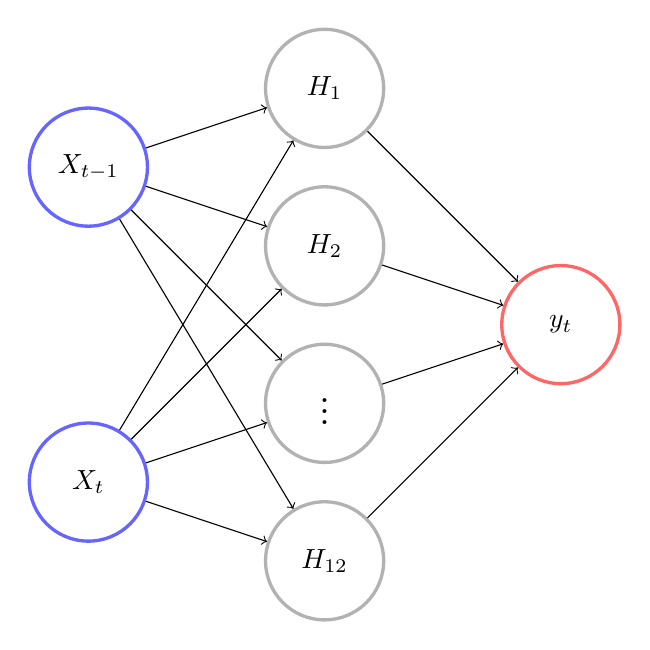
\begin{tikzpicture}[
            neuron/.style={circle, very thick, minimum size=15mm},
            input/.style={draw=blue!60},
            hidden/.style={draw=gray!60},
            output/.style={draw=red!60},]

        % Nodes entrada
        \node[neuron, input]  (entrada1)   at (0, 5cm)   {$X_{t-1}$};
        \node[neuron, input]  (entrada2)   at (0, 1cm)   {$X_{t}$};

        % Nodes escondidos
        \node[neuron, hidden] (escondido1) at (3cm, 6cm) {$H_1$};
        \node[neuron, hidden] (escondido2) at (3cm, 4cm) {$H_2$};
        \node[neuron, hidden] (escondido3) at (3cm, 2cm) {$\LARGE{\vdots}$};
        \node[neuron, hidden] (escondido4) at (3cm, 0)   {$H_{12}$};

        % Nodes Saída
        \node[neuron, output] (saida)      at (6cm, 3cm) {$y_t$};

        \foreach \dest in {1,...,4}
            \path[->] (entrada1) edge (escondido\dest);

        \foreach \dest in {1,...,4}
            \path[->] (entrada2) edge (escondido\dest);

        \foreach \dest in {1,...,4}
            \path[->] (escondido\dest) edge (saida);
    \end{tikzpicture}
    \source{Elaborado pelo autor}
\end{figure}

\postextual

\bibliography{referencias}

\end{document}
